\section*{Feuer machen}

\textbf{\Large Zur Sicherheit}\\
Wähle eine geeignete Feuerstelle, die weit genug entfernt von brennbarem Material ist (trockenes Gras, Heu, trockene Bäume).
Wenn du Feuer auf einer Wiese machst, hebe einige Grasziegel aus (bei Trockenheit wässern), damit du die Graswurzeln nicht verbrennst.\\
\textbf{Halte die Feuerstelle sauber, damit sich das Feuer nicht auf herumliegendes, brennbares Material ausweitet! Lasse dein Feuer nie unbeaufsichtigt!}

\textbf{\Large Brennmaterial sammeln}\\
Weiches, dünnes Holz zum Anbrennen (Birke, Fichte, Kiefer), Hartholz für lange Brenndauer und Glut (Ahorn, Eiche, Buche).\\
Wenn du kein Papier zum Anzünden hast, eignet sich Birkenrinde von toten(!) Bäumen besonders gut, alternativ kannst du auch dünne Späne schnitzen.

\textbf{\Large Feuer anzünden}\\
Baue dein Feuer in der beliebigen Form auf, unten den Unterzünder (Papier, Holzspäne), dann das dünne und zuletzt das dicke Holz.
Lass ausreichend Luft, damit der Wind das Feuer mit Sauerstoff versorgen kann.
Auf der Windseite lässt du eine Öffnung zum Anzünden.\\
Wenn du das Feuer anzündest, schirmst du den Wind so lange mit dem Körper ab, bis es so groß ist, dass der Wind die Flammen nicht mehr ausblasen kann.\\
Lege regelmäßig und rechtzeitig Holz nach, um das Feuer am Brennen zu halten.\\
Nasses Holz kannst du in der Nähe des Feuers trocknen, achte darauf, dass es nicht anbrennt.
\textbf{Verlasse die Feuerstelle erst, wenn das Feuer ganz ausgebrannt ist!}

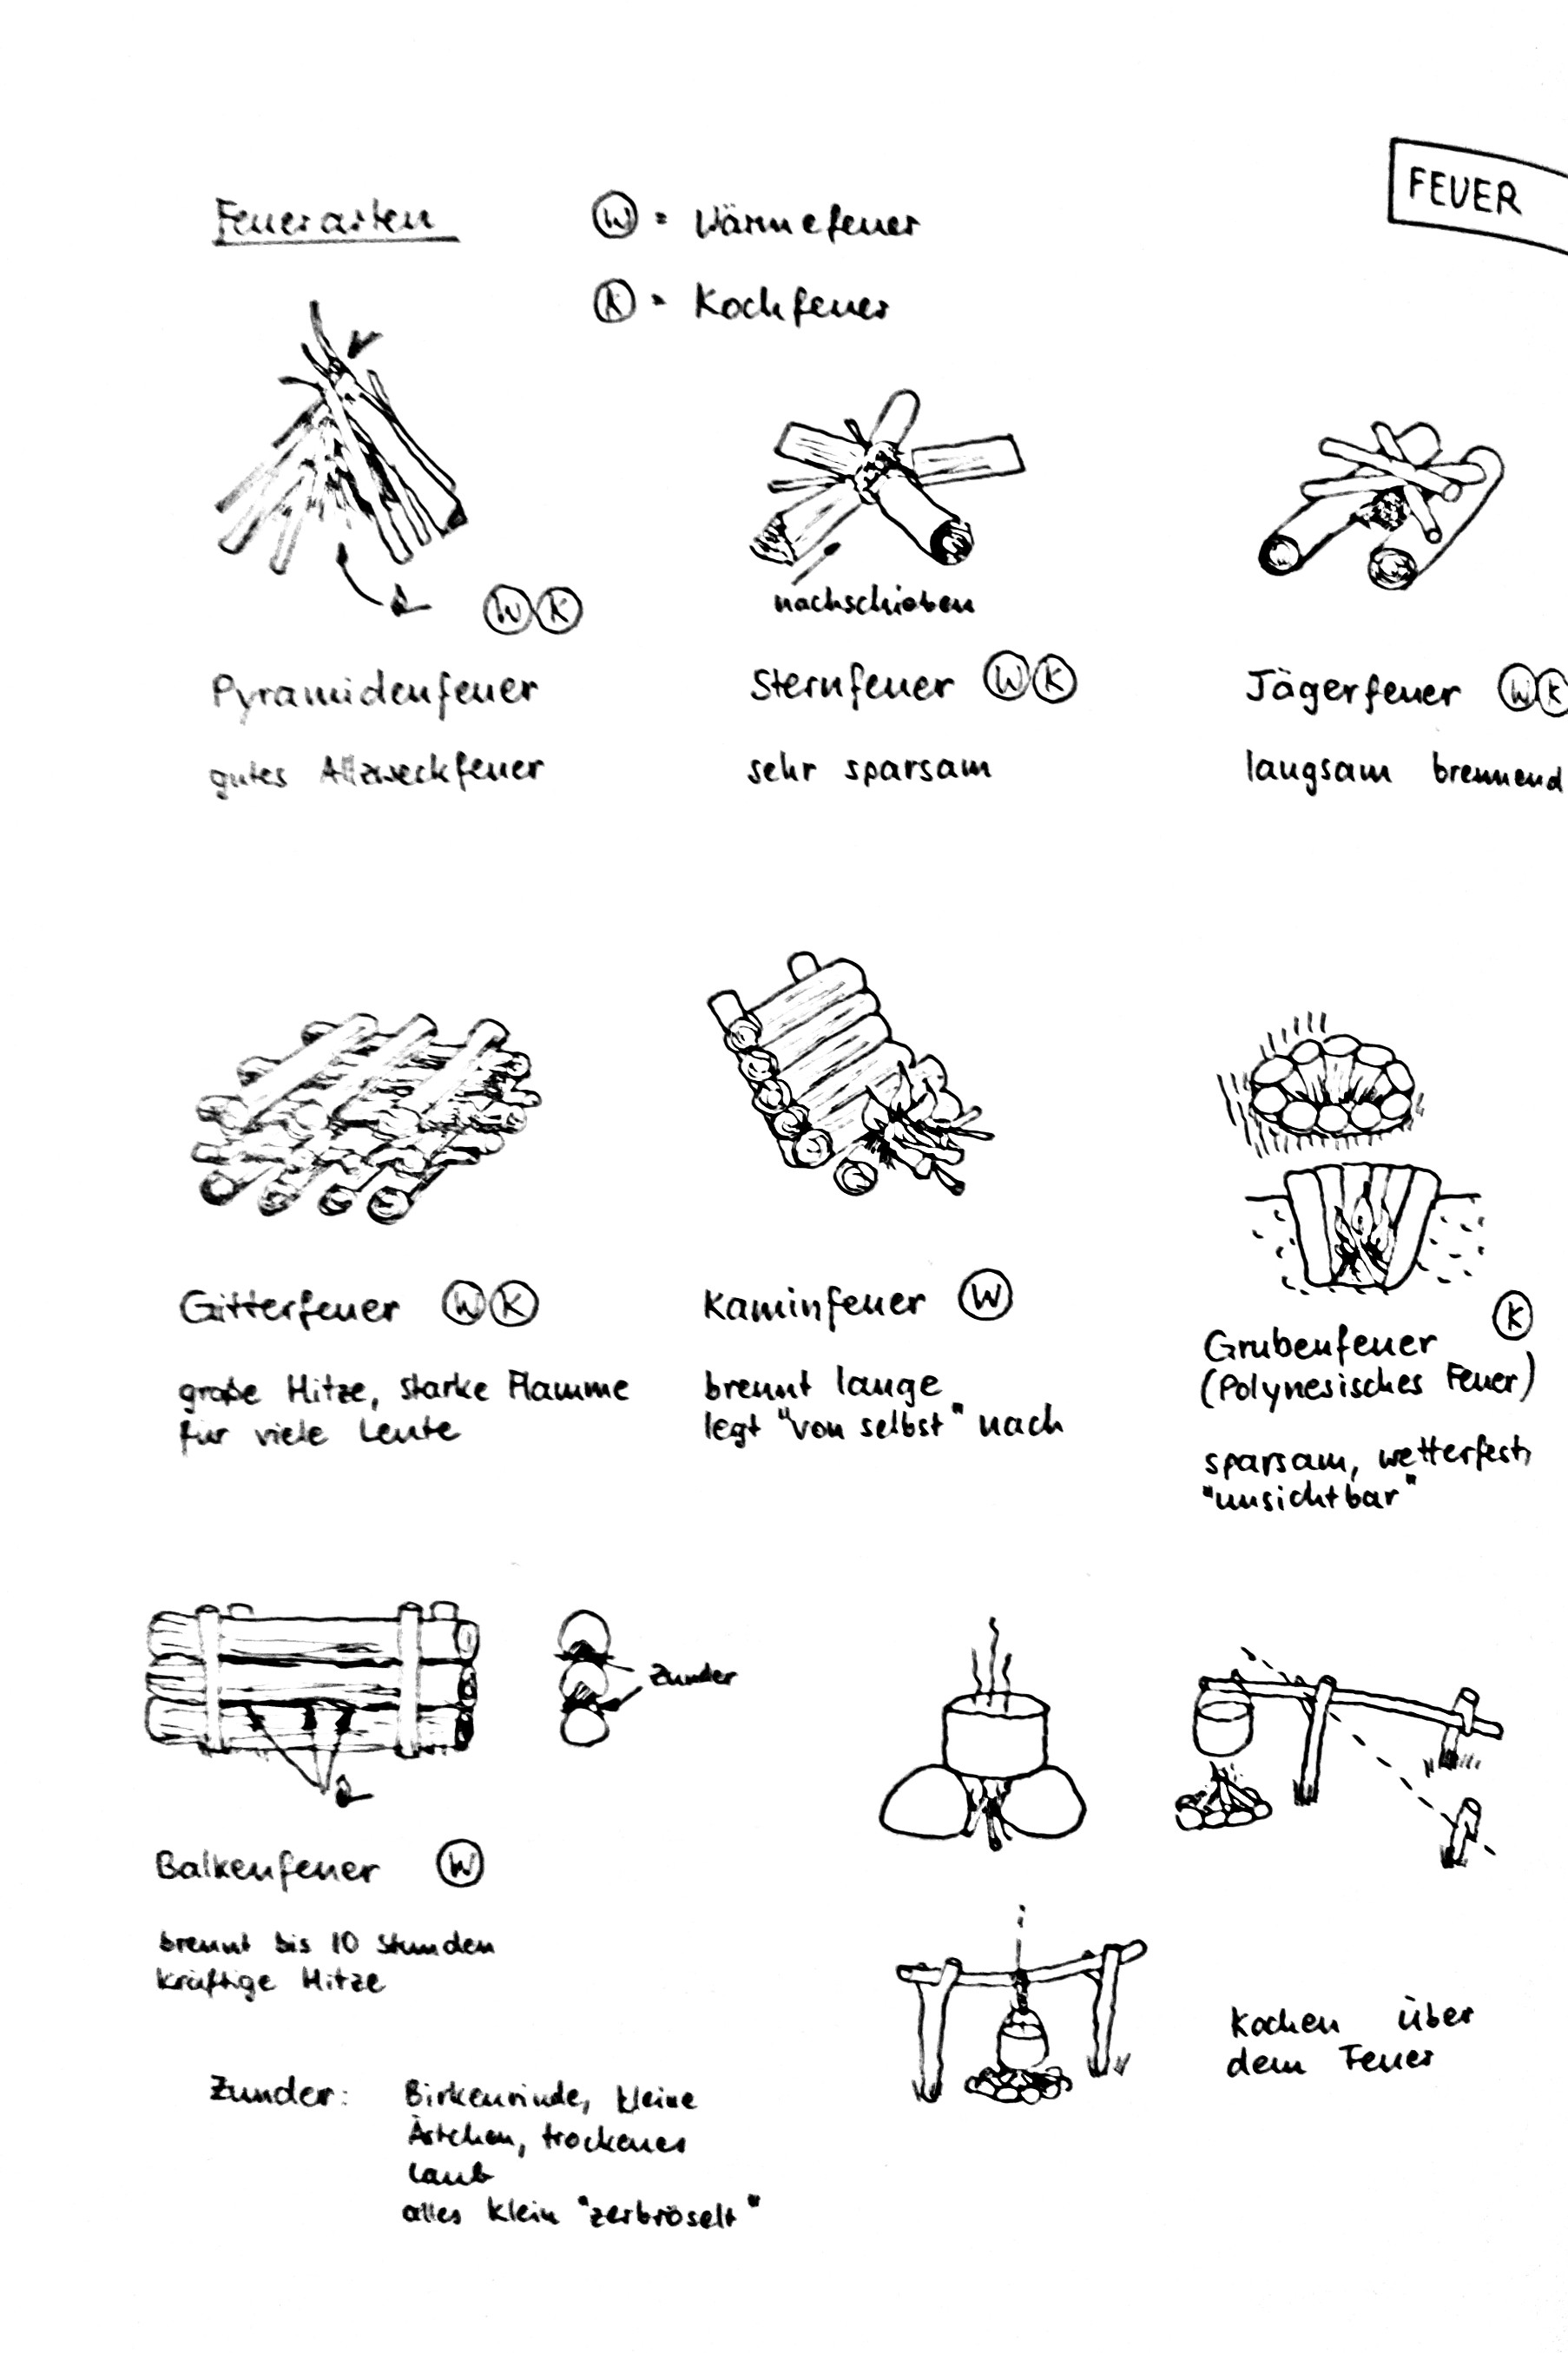
\includegraphics[width=\textwidth,height=\textheight,keepaspectratio]{Ausgaben/Sola24/Grafiken/Feuer.jpg}